\documentclass[12pt]{article}
\usepackage[spanish]{babel}
\usepackage{graphicx}
\usepackage{float}
\usepackage{listings}
\usepackage{xcolor}

\definecolor{codegreen}{rgb}{0,0.6,0}
\definecolor{codegray}{rgb}{0.5,0.5,0.5}
\definecolor{codepurple}{rgb}{0.58,0,0.82}
\definecolor{backcolour}{rgb}{0.95,0.95,0.92}


\lstdefinestyle{mystyle}{
	backgroundcolor=\color{backcolour},   
	commentstyle=\color{codegreen},
	keywordstyle=\color{magenta},
	numberstyle=\tiny\color{codegray},
	stringstyle=\color{codepurple},
	basicstyle=\ttfamily\footnotesize,
	breakatwhitespace=false,         
	breaklines=true,                 
	captionpos=b,                    
	keepspaces=true,                 
	numbers=left,                    
	numbersep=5pt,                  
	showspaces=false,                
	showstringspaces=false,
	showtabs=false,                  
	tabsize=2
}

\lstset{style=mystyle}

\title{Síntesis de redes activas \\ Laboratorio Nº4: Filtros Activos}

\author{Profesor Titular: Dr. Ing. Pablo Ferreyra \\  Profesor Adjunto: Ing. César Reale \\ Alumnos: Campos Mariano, 
	Enzo Verstraete}

\begin{document}
	\maketitle
	
	\begin{abstract}
		En base a la planilla de requerimientos suministrada, sintetizar un circuito basado en
		amplificadores operacionales que satisfaga esos requisitos.
	\end{abstract}\newpage
	
	
	\section{Metodología general}	
	En general, para cada uno de los casos particulares solicitados, se debe:
	A. Realizar una sintética introducción teórica.
	B. Analizar el circuito propuesto, su desarrollo numérico, todos los cálculos analíticos.
	C. Realizar simulación en LTSPICE.
	D. Armar el circuito y hacer las mediciones en laboratorio.
	E. Finalmente comparar los valores calculados, simulados y medidos, y extraer conclusiones a
	cerca de las diferencias. Analizar las causas.
	F. Presentar un informe digital y en papel.
	
	\section{Desarrollo}
	1.1 Aproximar la función de atenuación mediante polinomios de Chebychev utilizando python
	o matlab (ver Anexo I y II).
	1.2 Sintetizar un circuito que satisfaga los requerimientos del punto anterior utilizando topologías
	bicuadráticas de realimentación positiva o negativa, a elección.
	1.3 Simular cada etapa y el filtro total con LTSPICE.
	1.4 Calcular la sensibilidad de la frecuencia del polo de cada bicuadrática (wp) y del ancho de
	banda (wp/Qp).
	1.5 Analizar la peor desviación si todos los elementos tienen una tolerancia del 10 %.
	1.6 Realizar una simulación de Montecarlo de las desviaciones con LTspice.
	1.7 Armar el circuito, medir experimentalmente las curvas de atenuación y desfasaje. Contrastarlas
	con las predicciones teóricas y las simulaciones.
	
	\subsection{Aproximación de la función de transferencia}
	Para la aproximación del la función utilizamos el siguiente código en Matlab, partimos de los parámetros de diseño, en este caso tenemos un filtro pasa banda con las siguientes características:

	\begin{lstlisting}
		Parametros:
		Fbp = [800 1250]; % Puntos en frecuencia de la banda de paso entre 800 y 1250 [Hz]
		Fbr = [200 5000]; % Puntos en frecuencia de la banda de rechazo 0-200 [Hz] y 5000-inf [Hz]
		Wbp = 2*pi*Fbp;   % Puntos de omega [rad/s]
		Wbr = 2*pi*Fbr;   % Puntos en omega [rad/s]
		Abp = 0.25;       % Atenuacion en la banda de paso [dB]
		Abr = 30;         % Atenuacion en la banda de rechazo [dB]
		
	\end{lstlisting}
	
	El segundo paso es obtener la función de transferencia, por medio de la aproximación Chebychev  de primer orden:
	\begin{lstlisting}
		TF:
		[n , Wp] = cheb1ord(Wbp,Wbr,Abp,Abr,"s");  % Determinacion del orden y la frecuencia de corte de un filtro de chebyshev tipo 1
		[num , den] = cheby1(n,Abp,Wp,"s");        % Determinacion del numerador y denominador de la funcion de transferencia del filtro
		TF_filtro = tf(num,den);                   % Creacion de la TF del filtro
		
		% Descomposicion en bicuadraticas (debemos descomponer en una funcion para
		% filtro pasa-alto y otra para el filtro pasa-bajo):
		[Msos , Gg] = tf2sos(num,den);             % Descompone en bicuadraticas
		% Msos: matriz de coeficientes de la bicuadraticas ; Gg: ganancia global del filtro
		TFpb = tf(Gg*Msos(1,1:3) , Msos(1,4:6)); % Funcion de transferencia del filtro pasa-bajo
		% 2*Gg*Msos(1,1:3): coeficiente del numerador escalados por la ganancia global, Msos(1,4:6): coeficiente del denominador
		TFpa = tf(Msos(2,1:3) , Msos(2,4:6));  % Funcion de transferencia del filtro pasa-alto
		% 1/2*Msos(2,1:3): Coeficientes del numerador escalados por la ganancia global, Msos(2,4:6): Coeficientes del denominador
		
		figure                    % Diagramas de bode juntos
		hold on;
		bode(TF_filtro);
		bode(TFpa);
		bode(TFpb);
		hold off;
	\end{lstlisting}
	 
	 Obteniéndose como resultado las dos funciones transferencias, el filtro pasa bajo y filtro pasa alto, la suma resulta el pasa banda que estamos buscando:
	 
	\begin{figure}[h!]
		\includegraphics[width=1\linewidth]{"Simulaciones_Imagenes/funciones de transferencias"}
		\caption[Funciones de transferencias: Global, FPB, FPA]{Funciones de transferencias: Global, FPB, FPA}
		\label{fig:funciones-de-transferencias}
	\end{figure}
	
	\begin{figure}[h!]
		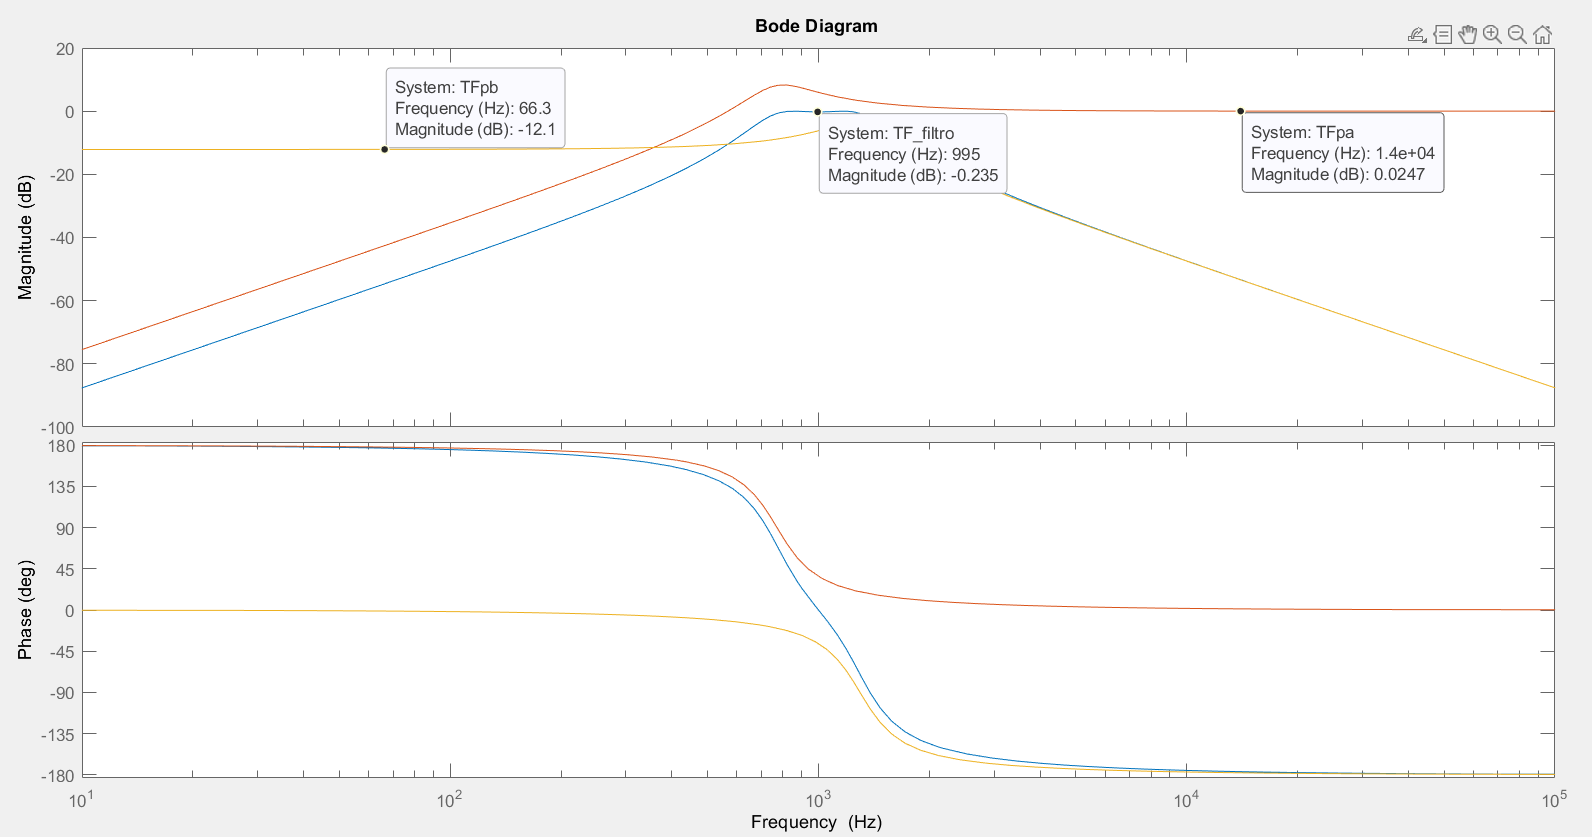
\includegraphics[width=1\linewidth]{Simulaciones_Imagenes/Bode_TFs_Matlab}
		\caption[Diagrama de bode: Global,FPB,FPA]{Diagrama de bode: Global,FPB,FPA}
		\label{fig:bodetfsmatlab}
	\end{figure}
	
	\subsection{Síntesis del filtro}
	A continuación se compara con las expresiones canónicas de los filtros para calcular los coeficientes, esto nos permite obtener los valores de resistencias y capacitancias
	\begin{lstlisting}
		Filtro pasa bajo:
		[num_pb,den_pb] = tfdata(TFpb);                % Obtencion numerador y denominador de la TFpb
		num_pb = cell2mat(num_pb);
		num_pb = num_pb(3);
		den_pb = cell2mat(den_pb);
		[Kpb,Wpb,Qpb] = obt_coef(num_pb,den_pb);       % Obtencion de K, W y Q
		
		% Tomamos R1 = R2 = 10000
		syms C1pb C2pb;
		R1pb = 10000;                                                 % Suponemos R1 para el FPB
		R2pb = 10000;                                                 % Suponemos R2 para el FPB
		eq1 = 1/(sqrt(C1pb*C2pb*R1pb*R2pb)) == Wpb;                   % Describimos la EC1
		eq2 = sqrt(C1pb/C2pb)*(sqrt(R1pb*R2pb)/(R1pb+R2pb)) == Qpb;   % Describimos la EC2
		solu1 = solve([eq1,eq2],[C1pb,C2pb]);                         % Obtenemos las soluciones de las ECs
		
		C1_pb = double(solu1.C1pb(2));                                % Valor de C1
		C2_pb = double(solu1.C2pb(2));                                % Valor de C2
		
		% El K lo hacemos con un divisor resistivo
		
		Filtro pasa alto:
		[num_pa,den_pa] = tfdata(TFpa);
		num_pa = cell2mat(num_pa);
		num_pa = num_pa(1);
		den_pa = cell2mat(den_pa);
		[Kpa,Wpa,Qpa] = obt_coef2(num_pa,den_pa);
		
		
		syms R1pa R2pa;
		C1pa = 0.0000001;
		C2pa = 0.0000001;
		eq3 = 1/(sqrt(C1pa*C2pa*R1pa*R2pa)) == Wpa;
		eq4 = 1/((sqrt(R1pa/R2pa)*((C1pa+C2pa)/sqrt(C1pa*C2pa)))+((1-Kpa)*sqrt((R2pa*C2pa)/(R1pa*C1pa)))) == Qpa;
		solu2 = solve([eq3,eq4],[R1pa,R2pa]);
		
		R1_pa = double(solu2.R1pa(2));
		R2_pa = double(solu2.R2pa(2));
		
	\end{lstlisting}
	
	Como resultado del análisis tenemos que los valores de R y C para el filtro pasa bajo son $R1=R2=10[Kohm]$ y los valores de capacidad $C1=62.8[nF]$ $C2=2.4[nF]$.Para el filtro pasa
	alto tenemos $C1=C2=10[uF]$ y para las resistencias $R1=400[ohm]$ $R2=10[Kohm]$. Por ultimo para 
	la síntesis del filtro se eligió la siguiente configuración: 
	  
	\begin{figure}[h!]
		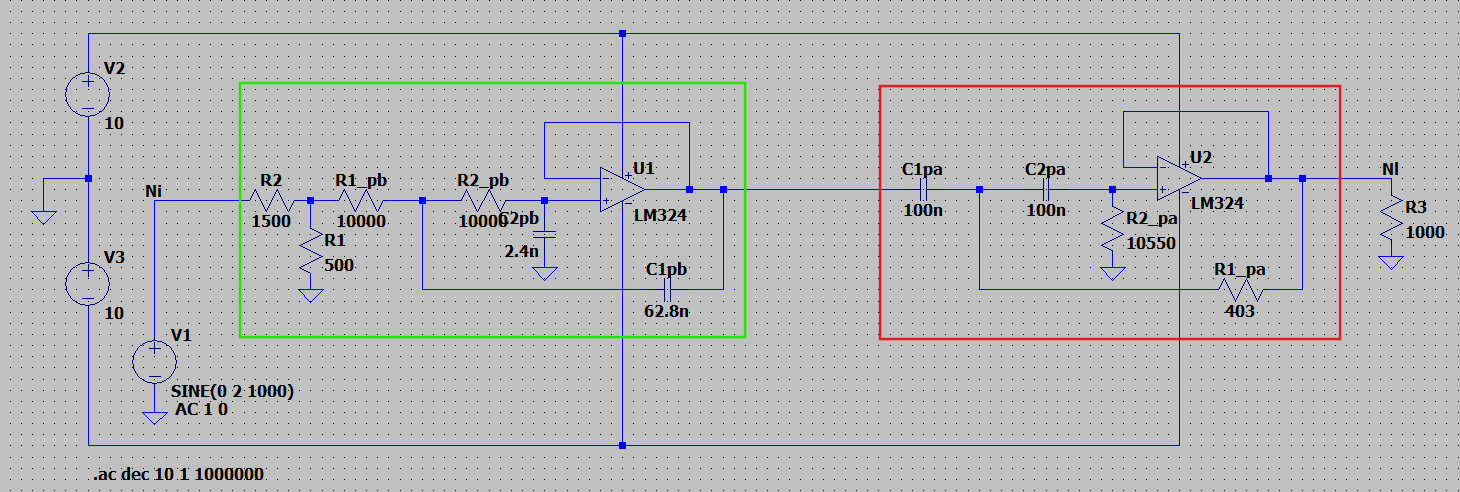
\includegraphics[width=1\linewidth]{Simulaciones_Imagenes/Circ_Filtro_VerdeFpb_RojoFpa}
		\caption[Síntesis del filtro pasa-banda]{Síntesis del filtro pasa-banda FPB+FPA}
		\label{fig:circfiltroverdefpbrojofpa}
	\end{figure}
	
	Por ultimo se verifican los resultados de modulo y fase con una simulación en LTSPICE
	\begin{figure}[h!]
		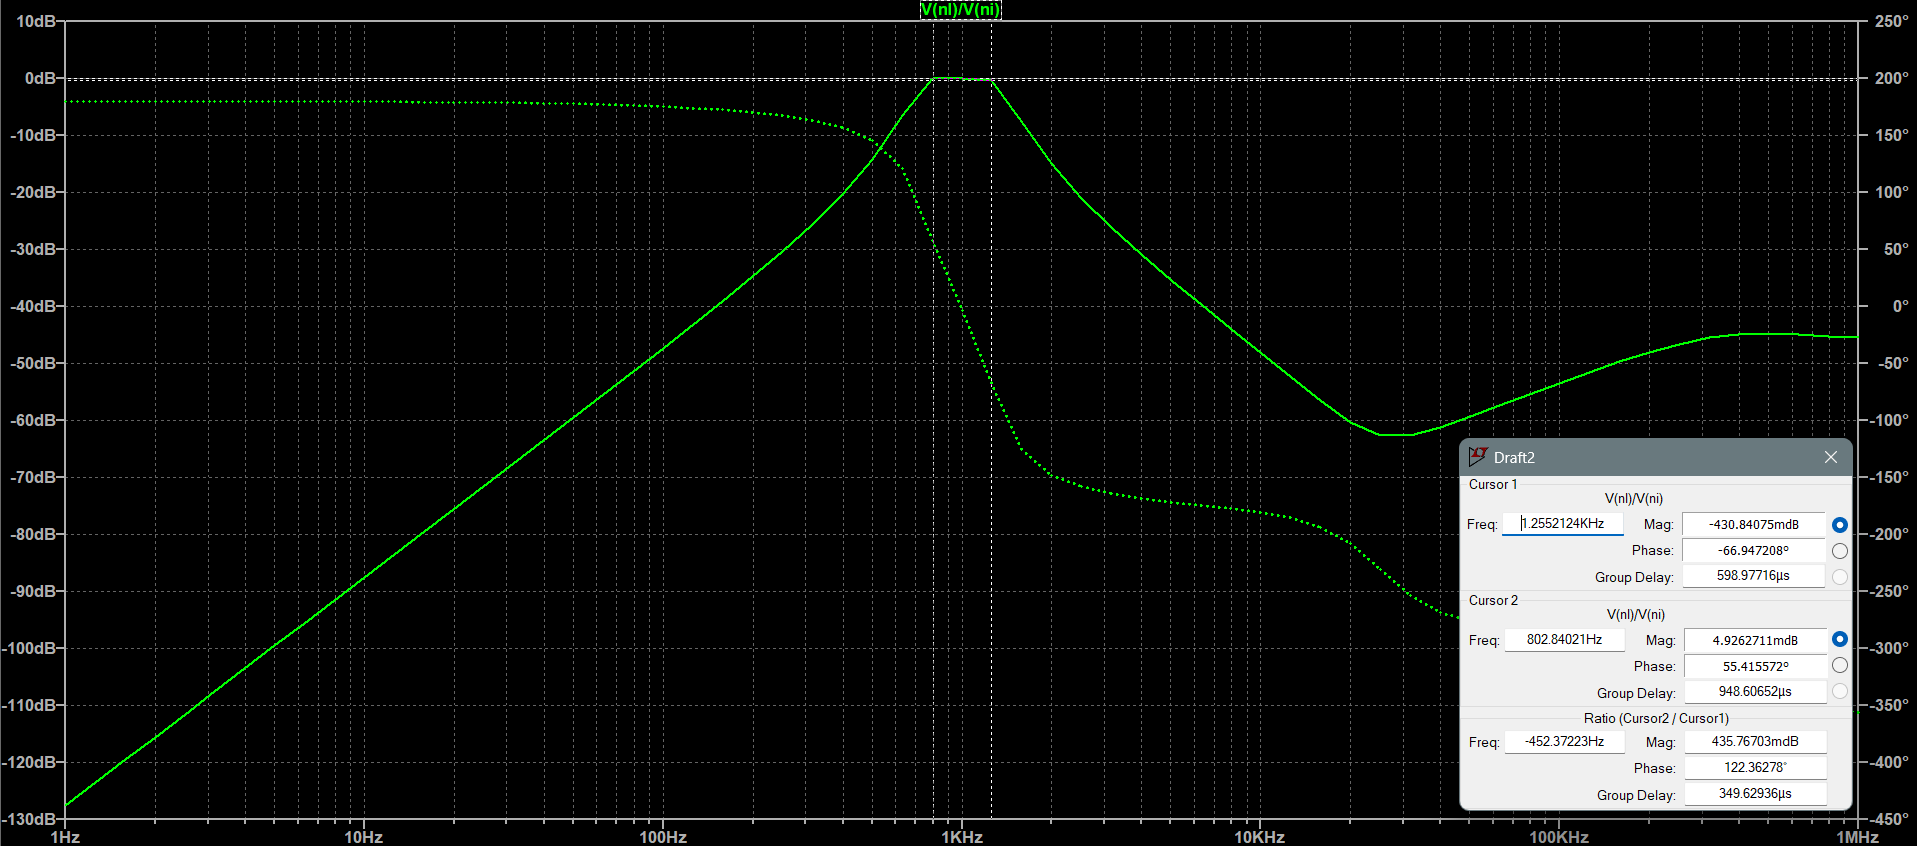
\includegraphics[width=1\linewidth]{Simulaciones_Imagenes/Sim_AC_Filtro}
		\caption[Respuesta en frecuencia del filtro]{Respuesta en frecuencia del filtro}
		\label{fig:simacfiltro}
	\end{figure}\newpage
	
	\subsection{Análisis de sensibilidad}
	El análisis de sensibilidad en el diseño de filtros activos es crucial porque evalúa cómo las variaciones en los parámetros de los componentes afectan el desempeño del circuito. Dado que los filtros activos están construidos con resistencias, capacitores, y amplificadores operacionales, las imperfecciones o desviaciones de estos elementos pueden alterar las características del filtro, como la frecuencia de corte, el factor de calidad, y la ganancia.
	
	Partimos del análisis de sensibilidad para el filtro pasa bajo, la expresión general del filtro es:
	\begin{equation}
		FPB(s)=\frac{K }{s^2+\frac{wp}{Qp}s+wp^2}
	\end{equation}
	La definición de sensitividad es:
	\begin{equation}
		S^p_{x}=\frac{x}{p}\frac{dp}{dx}
	\end{equation}
	
	Donde $p$ es el parámetro y $x$ es la variable.Teniendo en cuenta el circuito anterior mente presentados, podemos calcular la sensitividad para $wp$ y $wp/Qp$ con el siguiente script de matlab:
	 
	 \begin{lstlisting}
	 	%%Filtro pasa bajo
	 	% Declarar las variables simbolicas
	 	syms R1 R2 C1 C2
	 	% Definir la ecuacion para wp
	 	wp = sqrt(1 / (R1 * R2 * C1 * C2))
	 	% Sensibilidades de wp respecto a R1, R2, C1 y C2
	 	S_R1_wp = (R1 / wp) * diff(wp, R1);
	 	S_R2_wp = (R2 / wp) * diff(wp, R2);
	 	S_C1_wp = (C1 / wp) * diff(wp, C1);
	 	S_C2_wp = (C2 / wp) * diff(wp, C2);
	 	% Simplificar las sensibilidades
	 	S_R1_wp = simplify(S_R1_wp);
	 	S_R2_wp = simplify(S_R2_wp);
	 	S_C1_wp = simplify(S_C1_wp);
	 	S_C2_wp = simplify(S_C2_wp);
	 	% Definir la ecuacion para wp/Qp
	 	wp_Qp = (1 / (R1 * C1)) + (1 / (R2 * C1))
	 	% Sensibilidades de wp/Qp respecto a R1, R2, C1 y C2
	 	S_R1_wp_Qp = (R1 / wp_Qp) * diff(wp_Qp, R1);
	 	S_R2_wp_Qp = (R2 / wp_Qp) * diff(wp_Qp, R2);
	 	S_C1_wp_Qp = (C1 / wp_Qp) * diff(wp_Qp, C1);
	 	S_C2_wp_Qp = (C2 / wp_Qp) * diff(wp_Qp, C2);
	 	% Simplificar las sensibilidades
	 	S_R1_wp_Qp = simplify(S_R1_wp_Qp);
	 	S_R2_wp_Qp = simplify(S_R2_wp_Qp);
	 	S_C1_wp_Qp = simplify(S_C1_wp_Qp);
	 	S_C2_wp_Qp = simplify(S_C2_wp_Qp);
	 	% Valores especificos
	 	R1_val = 10e3; % 10 kOhm
	 	R2_val = 10e3; % 10 kOhm
	 	C1_val = 62.8e-9; % 62.8 nF
	 	C2_val = 2.4e-9; % 2.4 nF
	 	% Evaluar wp y wp/Qp numericamente
	 	wp_val = sqrt(1 / (R1_val * R2_val * C1_val * C2_val));
	 	wp_Qp_val = (1 / (R1_val * C1_val)) + (1 / (R2_val * C1_val));
	 	% Evaluar sensibilidades numericas de wp
	 	S_R1_wp_val = subs(S_R1_wp, [R1, R2, C1, C2], [R1_val, R2_val, C1_val, C2_val]);
	 	S_R2_wp_val = subs(S_R2_wp, [R1, R2, C1, C2], [R1_val, R2_val, C1_val, C2_val]);
	 	S_C1_wp_val = subs(S_C1_wp, [R1, R2, C1, C2], [R1_val, R2_val, C1_val, C2_val]);
	 	S_C2_wp_val = subs(S_C2_wp, [R1, R2, C1, C2], [R1_val, R2_val, C1_val, C2_val]);
	 	% Evaluar sensibilidades numericas de wp/Qp
	 	S_R1_wp_Qp_val = subs(S_R1_wp_Qp, [R1, R2, C1, C2], [R1_val, R2_val, C1_val, C2_val]);
	 	S_R2_wp_Qp_val = subs(S_R2_wp_Qp, [R1, R2, C1, C2], [R1_val, R2_val, C1_val, C2_val]);
	 	S_C1_wp_Qp_val = subs(S_C1_wp_Qp, [R1, R2, C1, C2], [R1_val, R2_val, C1_val, C2_val]);
	 	S_C2_wp_Qp_val = subs(S_C2_wp_Qp, [R1, R2, C1, C2], [R1_val, R2_val, C1_val, C2_val]);
	 	% Mostrar resultados numericos
	 	fprintf('\nSensibilidades numericas de wp:\n');
	 	fprintf('S_R1_wp = %.2f\n', double(S_R1_wp_val));
	 	fprintf('S_R2_wp = %.2f\n', double(S_R2_wp_val));
	 	fprintf('S_C1_wp = %.2f\n', double(S_C1_wp_val));
	 	fprintf('S_C2_wp = %.2f\n', double(S_C2_wp_val));
	 	fprintf('\nSensibilidades numericas de wp/Qp:\n');
	 	fprintf('S_R1_wp_Qp = %.2f\n', double(S_R1_wp_Qp_val));
	 	fprintf('S_R2_wp_Qp = %.2f\n', double(S_R2_wp_Qp_val));
	 	fprintf('S_C1_wp_Qp = %.2f\n', double(S_C1_wp_Qp_val));
	 	fprintf('S_C2_wp_Qp = %.2f\n', double(S_C2_wp_Qp_val));
	\end{lstlisting}
	
	Obteniéndose como resultado:
	\begin{figure}[h!]
		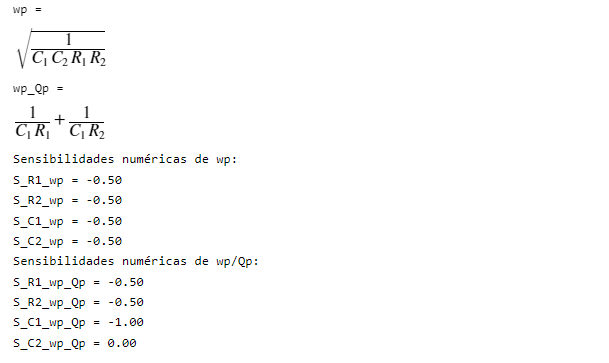
\includegraphics[width=1\linewidth]{Simulaciones_Imagenes/Sensitividad}
		\caption[Sensitividad filtro pasa bajo]{Sensitividad filtro pasa bajo}
		\label{fig:sensitividad}
	\end{figure}
	
	Realizando un estudio similar al anterior pero esta vez teniendo en cuenta la síntesis del filtro pasa alto, realizamos el análisis de sensibilidad:
	
	\begin{lstlisting}
		%%Filtro pasa alto:
		% Declarar las variables simbolicas
		syms R1 R2 C1 C2 k
		
		% Definir la ecuacion para wp
		wp = sqrt(1 / (R1 * R2 * C1 * C2))
		
		% Sensibilidades de wp respecto a R1, R2, C1 y C2
		S_R1_wp = (R1 / wp) * diff(wp, R1);
		S_R2_wp = (R2 / wp) * diff(wp, R2);
		S_C1_wp = (C1 / wp) * diff(wp, C1);
		S_C2_wp = (C2 / wp) * diff(wp, C2);
		
		% Simplificar las sensibilidades
		S_R1_wp = simplify(S_R1_wp);
		S_R2_wp = simplify(S_R2_wp);
		S_C1_wp = simplify(S_C1_wp);
		S_C2_wp = simplify(S_C2_wp);
		
		% Definir la ecuacion para wp/Qp con k = 1
		wp_Qp = -((k - 1) * sqrt((C2 * R2) / (C1 * R1)) - sqrt(R1 / R2) * (C1 + C2)) / sqrt(C1 * C2 * R1 * R2)
		
		% Sustituir k = 1 en la expresion
		wp_Qp = subs(wp_Qp, k, 1);
		
		% Sensibilidades de wp/Qp respecto a R1, R2, C1 y C2
		S_R1_wp_Qp = (R1 / wp_Qp) * diff(wp_Qp, R1);
		S_R2_wp_Qp = (R2 / wp_Qp) * diff(wp_Qp, R2);
		S_C1_wp_Qp = (C1 / wp_Qp) * diff(wp_Qp, C1);
		S_C2_wp_Qp = (C2 / wp_Qp) * diff(wp_Qp, C2);
		
		% Simplificar las sensibilidades
		S_R1_wp_Qp = simplify(S_R1_wp_Qp);
		S_R2_wp_Qp = simplify(S_R2_wp_Qp);
		S_C1_wp_Qp = simplify(S_C1_wp_Qp);
		S_C2_wp_Qp = simplify(S_C2_wp_Qp);
		
		% Nuevos valores especificos
		R1_val = 400; % 400 Ohm
		R2_val = 10e3; % 10 kOhm
		C1_val = 10e-6; % 10 uF
		C2_val = 10e-6; % 10 uF
		
		% Evaluar wp y wp/Qp numericamente
		wp_val = sqrt(1 / (R1_val * R2_val * C1_val * C2_val));
		wp_Qp_val = subs(wp_Qp, [R1, R2, C1, C2], [R1_val, R2_val, C1_val, C2_val]);
		
		% Evaluar sensibilidades numericas de wp
		S_R1_wp_val = subs(S_R1_wp, [R1, R2, C1, C2], [R1_val, R2_val, C1_val, C2_val]);
		S_R2_wp_val = subs(S_R2_wp, [R1, R2, C1, C2], [R1_val, R2_val, C1_val, C2_val]);
		S_C1_wp_val = subs(S_C1_wp, [R1, R2, C1, C2], [R1_val, R2_val, C1_val, C2_val]);
		S_C2_wp_val = subs(S_C2_wp, [R1, R2, C1, C2], [R1_val, R2_val, C1_val, C2_val]);
		
		% Evaluar sensibilidades numericas de wp/Qp
		S_R1_wp_Qp_val = subs(S_R1_wp_Qp, [R1, R2, C1, C2], [R1_val, R2_val, C1_val, C2_val]);
		S_R2_wp_Qp_val = subs(S_R2_wp_Qp, [R1, R2, C1, C2], [R1_val, R2_val, C1_val, C2_val]);
		S_C1_wp_Qp_val = subs(S_C1_wp_Qp, [R1, R2, C1, C2], [R1_val, R2_val, C1_val, C2_val]);
		S_C2_wp_Qp_val = subs(S_C2_wp_Qp, [R1, R2, C1, C2], [R1_val, R2_val, C1_val, C2_val]);
		
		% Mostrar resultados numericos
		fprintf('\nSensibilidades numericas de wp:\n');
		fprintf('S_R1_wp = %.2f\n', double(S_R1_wp_val));
		fprintf('S_R2_wp = %.2f\n', double(S_R2_wp_val));
		fprintf('S_C1_wp = %.2f\n', double(S_C1_wp_val));
		fprintf('S_C2_wp = %.2f\n', double(S_C2_wp_val));
		
		fprintf('\nSensibilidades numericas de wp/Qp:\n');
		fprintf('S_R1_wp_Qp = %.2f\n', double(S_R1_wp_Qp_val));
		fprintf('S_R2_wp_Qp = %.2f\n', double(S_R2_wp_Qp_val));
		fprintf('S_C1_wp_Qp = %.2f\n', double(S_C1_wp_Qp_val));
		fprintf('S_C2_wp_Qp = %.2f\n', double(S_C2_wp_Qp_val));
	\end{lstlisting}
	Los resultados obtenidos son los siguientes:
	\begin{figure}[h!]
		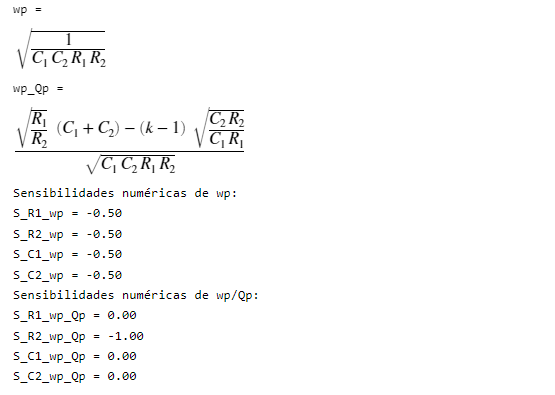
\includegraphics[width=1\linewidth]{Simulaciones_Imagenes/Sensitividad_2}
		\caption[Sensitividad filtro pasa alto]{Sensitividad filtro pasa alto}
		\label{fig:sensitividad2}
	\end{figure}
	
	\subsection{Simulación de Montecarlo}
	La simulación de Montecarlo es una técnica estadística que utiliza múltiples iteraciones para analizar cómo la variabilidad en los parámetros afecta el rendimiento de un sistema. En el caso de los filtros activos, esta técnica permite evaluar la sensibilidad y robustez del diseño frente a las imperfecciones en los componentes reales, como resistencias y capacitores.Montecarlo ayuda a simular miles de combinaciones posibles dentro de estas tolerancias y analiza el impacto de estas variaciones en parámetros clave del filtro, como la frecuencia de corte (wp), el factor de calidad (Qp), o la ganancia.
	
	En la simulación corremos 1000 veces sobre la variable $V(out)$ (distribución gaussiana) todos los componentes tienen una tolerancia del diez por ciento, con esto obtenemos los datos para el análisis.
	
	\begin{figure}
		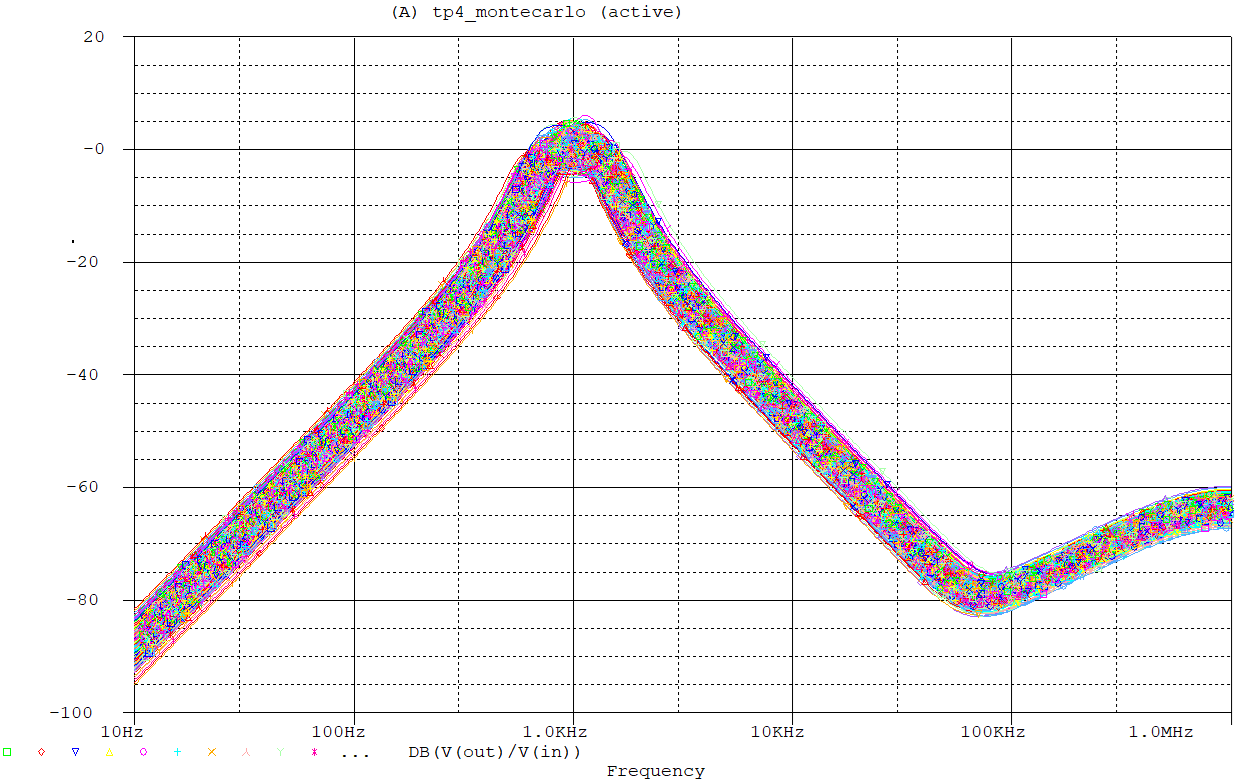
\includegraphics[width=1\linewidth]{Simulaciones_Imagenes/monte_carlo_1}
		\caption[Análisis de Montecarlo]{Análisis de Montecarlo}
		\label{fig:montecarlo1}
	\end{figure}
	
	Como tenemos un filtro pasa banda nos interesa hacer un análisis de rendimiento en la banda de paso, para eso utilizamos la siguiente función $Bandwidth3dB()$: Encuentre la diferencia entre los valores X donde la traza cruza primero su valor máximo menos 3 dB (Ymax-3dB) con una pendiente positiva y luego con una pendiente negativa. (es decir, encuentre el ancho de banda de 3 dB de una señal).
	
	\begin{figure}[h!]
		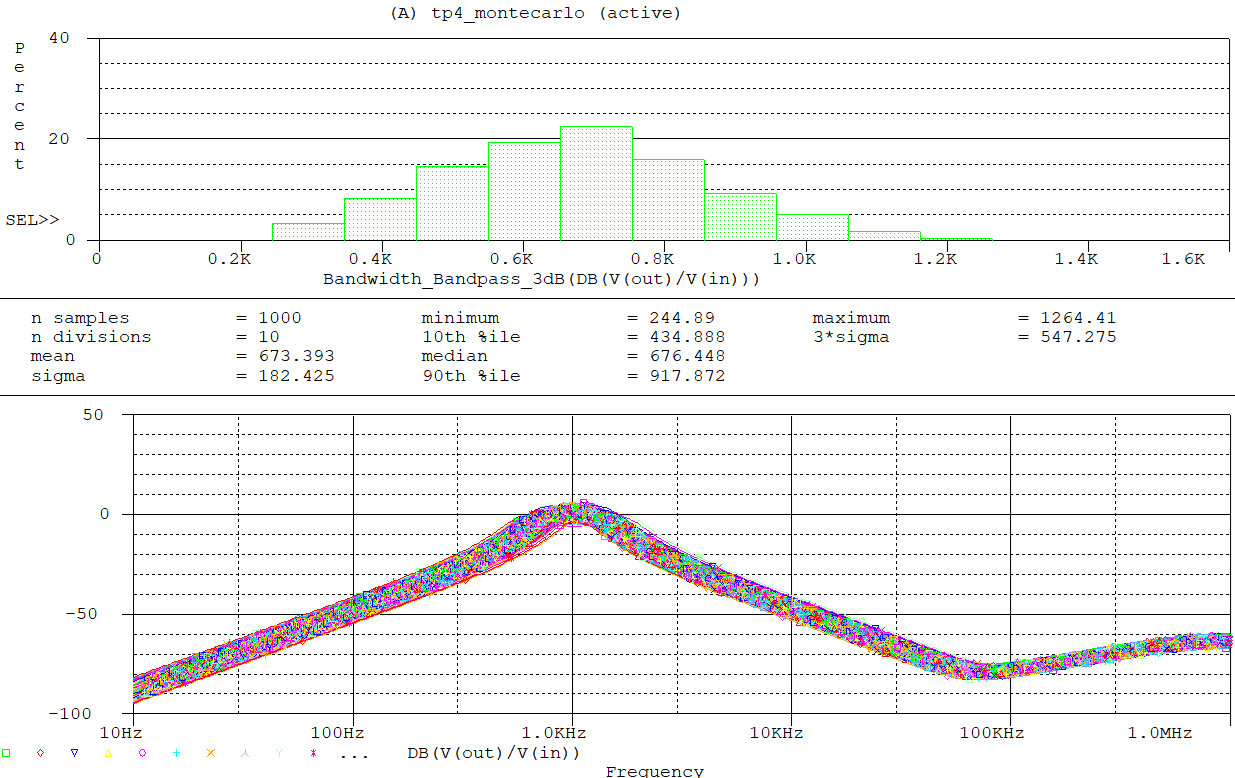
\includegraphics[width=1\linewidth]{Simulaciones_Imagenes/banda_de_paso_montecarlo}
		\caption[Análisis de banda de paso con Montecarlo]{Análisis de banda de paso con Montecarlo}
		\label{fig:bandadepasomontecarlo}
	\end{figure}
	
	\begin{figure}[h!]
		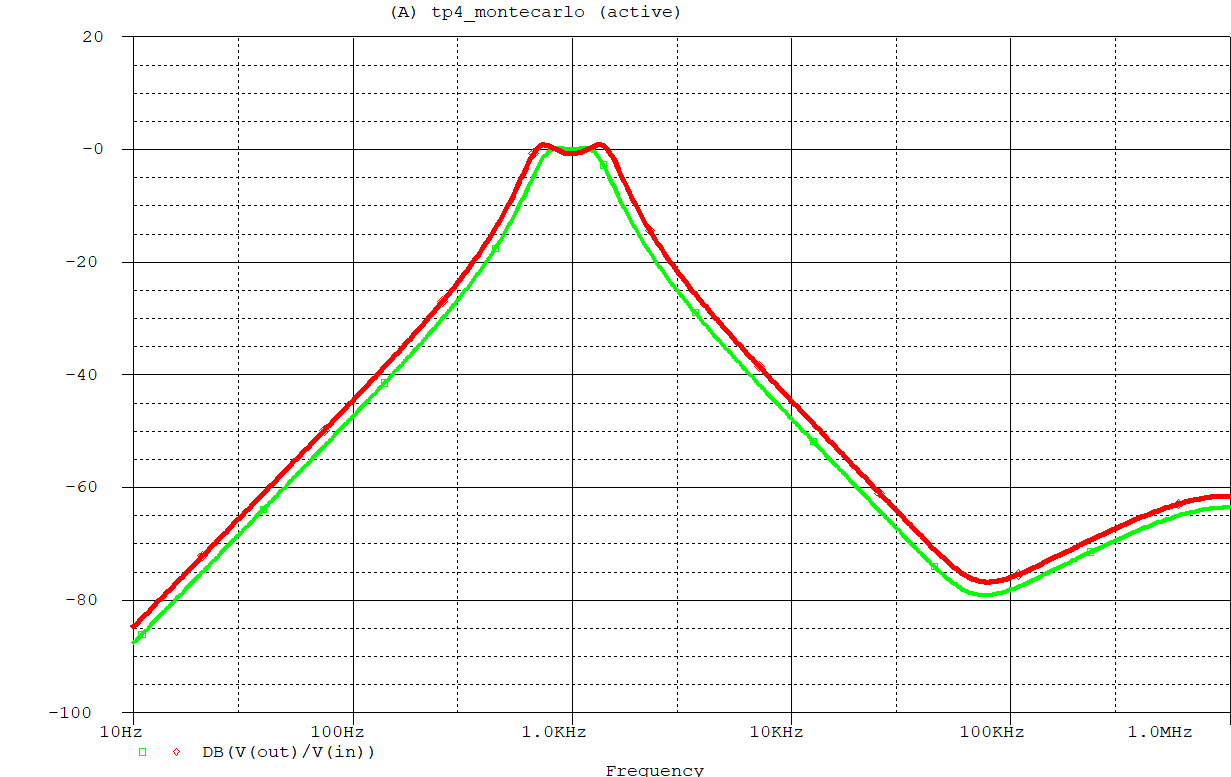
\includegraphics[width=1\linewidth]{Simulaciones_Imagenes/peor_de_los_casos}
		\caption[Análisis para el peor de los casos]{Análisis para el peor de los casos}
		\label{fig:peordeloscasos}
	\end{figure}
	
	
\end{document}
}